\documentclass{article}
\usepackage[utf8]{inputenc}
\usepackage{amsmath}
\usepackage{multicol}
\usepackage{multirow}
\usepackage{graphicx}

\title{Mixture model}
\author{Tawhidul Bhuiyan}
\date{May 2022}

\begin{document}

\maketitle

\section{Introduction}
\label{sec:into}
From Wikipedia, the free encyclopedia

\textit{Not to be confused with mixed model.}

\textit{See also: Mixture distribution}

In statistics, a mixture model is a probabilistic model for representing the presence of subpopulations within an overall population, without requiring that an observed data set should identify the sub-population to which an individual observation belongs. Formally a mixture model corresponds to the mixture distribution that represents the probability distribution of observations in the overall population. However, while problems associated with "mixture distributions" relate to deriving the properties of the overall population from those of the sub-populations, ``mixture models" are used to make statistical inferences about the properties of the sub-populations given only observations on the pooled population, without sub-population identity information.

Mixture models should not be confused with models for compositional data, i.e., data whose components are constrained to sum to a constant value (1, 100\%, etc.). However, compositional models can be thought of as mixture models, where members of the population are sampled at random. Conversely, mixture models can be thought of as compositional models, where the total size reading population has been normalized to 1.

\section{Multivariate Gaussian mixture model}
A Bayesian Gaussian mixture model is commonly extended to fit a vector of unknown parameters (denoted in bold), or multivariate normal distributions. In a multivariate distribution (i.e. one modelling a vector $\mathbf{x}$ with N random variables) one may model a vector of parameters (such as several observations of a signal or patches within an image) using a Gaussian mixture model prior distribution on the vector of estimates given by

\begin{equation}
\label{eq:1}
    p(\theta) = \sum_{i=1}^K \phi_{i} \mathcal{N}(\mu_i, \Sigma_i)
\end{equation}

Refer to section~\ref{sec:into}.

Refer to equation~\eqref{eq:1}.

\section{Math}
\subsection{Cases}
\begin{equation*}
    |x| = 
    \begin{cases}
    x & \text{if }x \geq 0 \\
    -x & \text{if}\ x < 0
    \end{cases}
\end{equation*}

\subsection{Align}
\begin{align}
    f(x) &= x^2-1 \nonumber \\
     &= (x-1)(x+1)
\end{align}

\section{Table}
\subsection{Tabular}
\begin{tabular}{|c|l|p{1cm}|}
\hline
col1 & col2 & col3 (in cm) \\
\hline
1 & 2 & 3\\
\hline
4 & 5 & 6 \\
\hline
\end{tabular}

\subsection{Multi-column}

\begin{tabular}{|c|c|c|}
\hline
col1 & \multicolumn{2}{|c|}{multicol} \\
\hline
1 & 2 & 3\\
\hline
4 & 5 & 6 \\
\hline
\end{tabular}

\begin{tabular}{|c|l|p{1cm}|}
\hline
col1 & col2 & col3 (in cm) \\
\hline
1 & 2 & \multicolumn{1}{|r|}{3}\\
\hline
4 & 5 & 6 \\
\hline
\end{tabular}

\subsection{Multi-row}
\begin{tabular}{|c|c|c|}
\hline
col1 & col2 & col3 (in cm) \\
\hline
\multirow{2}{*}{miltrow} & 2 & 3\\
\cline{2-3}
 & 5 & 6 \\
\hline
\end{tabular}

\subsection{Mixed}
\begin{tabular}{|cc|c|}
\hline
\multicolumn{2}{|c|}{\multirow{2}{*}{mixed}} & col3 \\
\cline{3-3}
 &  & 3\\
\hline
4 & 5 & 6 \\
\hline
\end{tabular}

\subsection{Table}
\begin{table}[h!]
    \centering
    \begin{tabular}{|c|c|c|}
    \hline
    col1 & col2 & col3 (in cm) \\
    \hline
    \multirow{2}{*}{miltrow} & 2 & 3\\
    \cline{2-3}
     & 5 & 6 \\
    \hline
    \end{tabular}
    \caption{Table}
    \label{tab:my_label}
\end{table}

\section{Figure}
\begin{figure}[p]
    \centering
    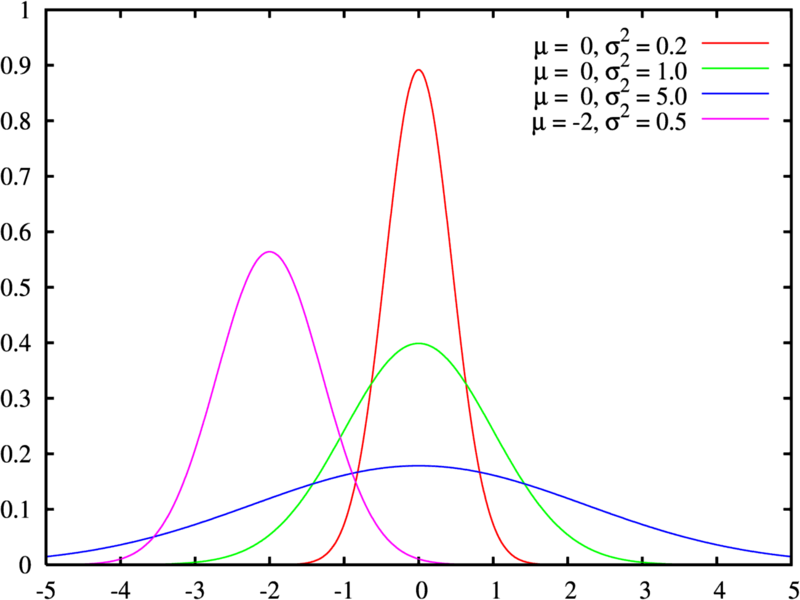
\includegraphics[width=0.5\textwidth]{Normal_distribution.png}
    \caption{Caption of Figure}
    \label{fig:my_label}
\end{figure}

\end{document}
